\documentclass[11pt]{report}

%using utf8
\usepackage[utf8]{inputenc}
\usepackage[english]{babel}

\usepackage[pdftex]{graphicx}

\usepackage{titlesec}

%embed urls
\usepackage{hyperref}
\usepackage{url}

%can use blind text
\usepackage{blindtext}

%improves the caption
\usepackage[font=it]{caption}

% to remove the number from the equations.
\usepackage{amsmath}

%Removes the Chapter from each chapter headline
\titleformat{\chapter}[block]
  {\normalfont\huge\bfseries}{\thechapter.}{1em}{\Huge}

\begin{document}

%%%%%%%%%%%%%%%%%%%%%%%%%%%%%%%%%%%%%%%%%
% University Assignment Title Page 
% LaTeX Template
% Version 1.0 (27/12/12)
%
% This template has been downloaded from:
% http://www.LaTeXTemplates.com
%
% Original author:
% WikiBooks (http://en.wikibooks.org/wiki/LaTeX/Title_Creation)
%
% License:
% CC BY-NC-SA 3.0 (http://creativecommons.org/licenses/by-nc-sa/3.0/)
% 
% Instructions for using this template:
% This title page is capable of being compiled as is. This is not useful for 
% including it in another document. To do this, you have two options: 
%
% 1) Copy/paste everything between \begin{document} and \end{document} 
% starting at \begin{titlepage} and paste this into another LaTeX file where you 
% want your title page.
% OR
% 2) Remove everything outside the \begin{titlepage} and \end{titlepage} and 
% move this file to the same directory as the LaTeX file you wish to add it to. 
% Then add \input{./title_page_1.tex} to your LaTeX file where you want your
% title page.
%
%%%%%%%%%%%%%%%%%%%%%%%%%%%%%%%%%%%%%%%%%

%----------------------------------------------------------------------------------------
%	PACKAGES AND OTHER DOCUMENT CONFIGURATIONS
%----------------------------------------------------------------------------------------

\begin{titlepage}

\newcommand{\HRule}{\rule{\linewidth}{0.5mm}} % Defines a new command for the horizontal lines, change thickness here

\center % Center everything on the page
 
%----------------------------------------------------------------------------------------
%	HEADING SECTIONS
%----------------------------------------------------------------------------------------

\includegraphics[width=0.15\textwidth]{./logo}\\[1cm]

\textsc{\LARGE Otto-von-Guericke University Magdeburg}\\[0.5cm] % Name of your university/college
\textsc{\large Faculty of Computer Science}\\[1.0cm] % Minor heading such as course title
\textsc{\Large Bachelor's Thesis}\\[1.0cm] % Major heading such as course name

%----------------------------------------------------------------------------------------
%	TITLE SECTION
%----------------------------------------------------------------------------------------

\HRule \\[0.5cm]
{ \huge \bfseries Interactive Visualization of Large Concept Lattices for Exploratory Search}\\[0.5cm] % Title of your document
\HRule \\[1.0cm]
 
%----------------------------------------------------------------------------------------
%	AUTHOR SECTION
%----------------------------------------------------------------------------------------

\Large \emph{Author:}\\
Johannes \textsc{Filter}\\[0.5cm]

\Large \emph{Advisors:}\\
Prof. Dr. Andreas \textsc{Nürnberger}\\
{\small Otto-von-Guericke University Magdeburg}\\[0.5cm]

Prof. Dr. Ana \textsc{García-Serrano}\\
{\small Universidad Nacional de Educación a Distancia}\\[1.0cm]

%----------------------------------------------------------------------------------------
%	DATE SECTION
%----------------------------------------------------------------------------------------

{\large \today}

\vfill % Fill the rest of the page with whitespace

\end{titlepage}

\renewcommand{\thepage}{\roman{page}}% Roman numerals for page counter

\newpage
\thispagestyle{empty}
\mbox{}

\chapter*{Abstract}
\blindtext

\newpage
\thispagestyle{empty}
\mbox{}

\chapter*{Inhaltsangabe}
\blindtext

\newpage
\thispagestyle{empty}
\mbox{}

\chapter*{Acknowledgements}
\blindtext

\newpage
\thispagestyle{empty}
\mbox{}

\tableofcontents
\newpage

\newpage
\thispagestyle{empty}
\mbox{}


\chapter{Introduction}

\renewcommand{\thepage}{\arabic{page}}
\setcounter{page}{1}

The digital revolution is affecting every part of our life. Also the humanities scholars stand before a big change in their ways when huge analog collections are digitized. They have to apply computer science methods to organize and analyze huge amount of data. The term "Digital Humanities" evolved during the last 10 years which can be defined as an "intersection between the humanities and information technology" \cite{Svensson2010}.\\

 The Information Retrieval Department of the Universidad Nacional de Educación a Distancia (UNED) in Madrid (Spain) cooperates with human scholars to conduct research in the Digital Humanities. In this project, there are historical maps which have been digitized and annotated. To extract knowledge from the collection the research group advocates for the use of Formal Concept Analysis (FCA) for topic organization \cite{Castellanos,Cigarran}.\\
 
 They successfully implemented a FCA algorithm but lack an interactive user interface which will be developed in this thesis. The work will be evaluated with an user study. \\
   
 While FCA is a mathematically well-funded principle, the resulting traditional visualization of large concept lattices are a problem. Large concept lattices arose when you apply FCA to large amount of entities (Details will be explained in Chapter 2). When applying FCA to a document collection, you are likely to occur huge amount of entities. That is why alternative visualization techniques are important to get the insights of FCA, even if the lattice is large. \\
  
 This thesis does not focus on the visualization of concept lattices itself. It focus on the visualization of concept lattices to explore and browse the data. This is different because it sets the data itself into the center and not the structure that was built around the data, the concept lattice.\\
 
This user interface will be web-based, to avoid dealing with setup problems you encounter when dealing with a heterogeneous operating systems environment. Because of the fast-changing environment of the web, it is important to keep with the latest technologies and techniques to not fall apart. Besides others, the software utilizes the frameworks d3.js and Bootstrap to create a pleasant user interface. The website is fast-responding because it reduces the communication between browser and web server to a minimum. In most cases, instead of reloading the page, the interface only changes DOM elements. \\
    
 The remainder of this thesis is structured as follows: The background of Formal Concept Analysis will be presented in Chapter 2 and the background of User Search Interfaces in Chapter 3. In Chapter 4 I will present my (first) approach and the implementation, which will be evaluated in Chapter 5. Built on the Evaluation, I will adjust my work and present an updated version of my work in Chapter 6. I conclude in Chapter 7 and give ideas for future work.
 
\chapter{Background}

Before we can analyze already existing work in this area, draw our conclusions and develop our own system, we have give background information. This chapter gives an introduction into formal concept analysis, followed by an introduction into user interface design principles.

\section{Formal Concept Analysis}

Formal Concept Analysis (FCA) is a mathematically well-funded technique to analyze data. FCA builds domain ontologies from object specified by attributes. It derives from old philosophical ideas and was formalized by Rudolf Wille \cite{Ganter2012}. \\

In the first section a small introduction is given and the second part the application for information retrieval are explained.

\subsection{Definition}

FCA is constructed from a formal context. A \textit{formal context} is defined as as a tripple $K = (G, M, I)$ where $G$ is a set of objects, $M$ is a set of attributes and $I$ is a binary relation $I \subseteq G \times M$. $I$ specifies whether an object has an attribute or not. ($G$ and $M$ come from the German words 'Gegenstand' and 'Merkmal'.) \\

Table \ref{table:example} illustrates an example (from David Eppstein \cite{fcaexample}) where $G$ comprises the integers from 1 to 10 and $M$ comprises the attributes composite, even, odd, prime and square. \\


\begin{table}[h]
\caption{Formal context, integers 1 to 10 as objects and attributes}
\label{table:example}
\centering

\def\arraystretch{1.2}% 
\begin{tabular}{ | c | c c c c c |}
\hline
  & composite & even & odd & prime & square\\
\hline

1 & & & $\times$ & &$\times$\\ 
2 & & $\times$ & & $\times$ &\\
3 & & & $\times$ & $\times$ &\\ 
4 & $\times$ & $\times$ & & & $\times$\\
5 & & & $\times$ & $\times$ &\\
6 & $\times$ & $\times$ & & &\\
7 & & & $\times$ & $\times$ &\\ 
8 & $\times$ & $\times$ & & &\\
9 & $\times$ & & $\times$ & & $\times$\\
10 & $\times$ & $\times$ & & &\\ \hline


\end{tabular}
\end{table}

Let the operator $'$ for $A \subseteq G$ be defined as following:
\begin{align*}
	A' = \{ m \subseteq M\; |\;  I(g, m)\;   \forall g \in A\}
\end{align*}

$A'$ is the set of those attributes that are present in all objects from given $A$. \\

Let the operator $'$ for $B \subseteq M$ be defined as following:
\begin{align*}
	B' = \{ g \subseteq G\; |\;  I(g, m)\;   \forall m \in B\}
\end{align*}

$B'$ is the set of objects that have at least the attributes given in $B$. \\

If for $A \subseteq G$ such that $A = A''$, then $A$ is called \textit{closed}. The same is true for $B \subseteq M$ and $B = B''$. \\

For example, let a set of objects be defined as $A_1 = \{1,4\} \subseteq G$. This results into: $A_1' = \{square\}$ and $A_1'' = \{1,4,9\}$. $A_1$ is not closed but $A_2 = {1,4,9} \subseteq G$ is called close because $A_2 = A_2''$. \\   

A \textit{formal concept} is a pair of $(A, B)$ where $A \subseteq G$ and $B \subseteq M$ and $A = B' \wedge B = A' $. Informally, all objects in $A$ share exactly the same attributes in $B$. $A$ is a set of objects called the \textit{extent} of a formal concept. $B$ a set of attributes called the \textit{intent} of a formal concept. The extent and the intent of all formal concepts are always closed.\\

From the example in \ref{table:example}, we can derive several formal concepts. Three randomly chosen concepts are shown in table \ref{table:exampleConcepts}. \\

\begin{table}[h]
\caption{Three formal concepts from the formal context in table \ref{table:example}}
\label{table:exampleConcepts}
\centering

\def\arraystretch{1.2}% 
\begin{tabular}{ c c c }
\hline
 Concept & Extent & Intent \\
\hline

$C_1$ & \{4,6,8,10\} & \{composite, even\} \\
$C_2$ & \{2,4,6,8,10\} & \{even\} \\
$C_3$ & \{9\} & \{composite, odd, square\} \\

\hline
\end{tabular}
\end{table}

It is possible to define an order relation on the formal concepts. Let us introduce the relation $\le$ as follows:
\begin{align*} (A_i,B_i) \le (A_j, B_j) \Longleftrightarrow	A_i \subseteq A_j
\end{align*}

With the help of $\le$, we  can derive relationships from the the concepts in table \ref{table:exampleConcepts}. We see that $C_1 \le C_2$. This means that $C_1$ is more specific than $C_2$ and $C_2$ is more general than $C_1$. We can also see that $C_3$ is unrelated to $C_1$, and that $C_3$ is unrelated to $C_2$. \\

A formal context with $\le$ is called a \textit{concept lattice} of the context. It can be shown, that for two formal concepts $C_i$ and $C_j$, there always exist a formal concept $C_x$ such that $C_i \le C_x \wedge C_j \le C_x$. So there exist always exist a formal concept wich is 'above' in the hierarchy and also related to the two formal concepts. \\ 

The interested reader is advices to read "The Basic Theorem on Concept Lattices" for instance in \cite{carpineto2004concept} for an formal explanation. \\

In the next section we will take a look at the static visualization of concept lattices.

\subsection{Static Visualization}

It is often said that a picture is worth a thousand words. To convey the abstract insights of a concept lattice, it can be visually represented in a \textit{Hasse diagram}. Figure \ref{figure:example} shows the Hasse diagram of the concept lattice derived from the formal context described in table \ref{table:example}. \\

\begin{figure*}[h]
\caption{Hasse diagramm, with the integers 1 to 10 as objects and attributes square (s), prime (p), composite (c), even (e), and odd (o)}
\label{figure:example}
	\centering
	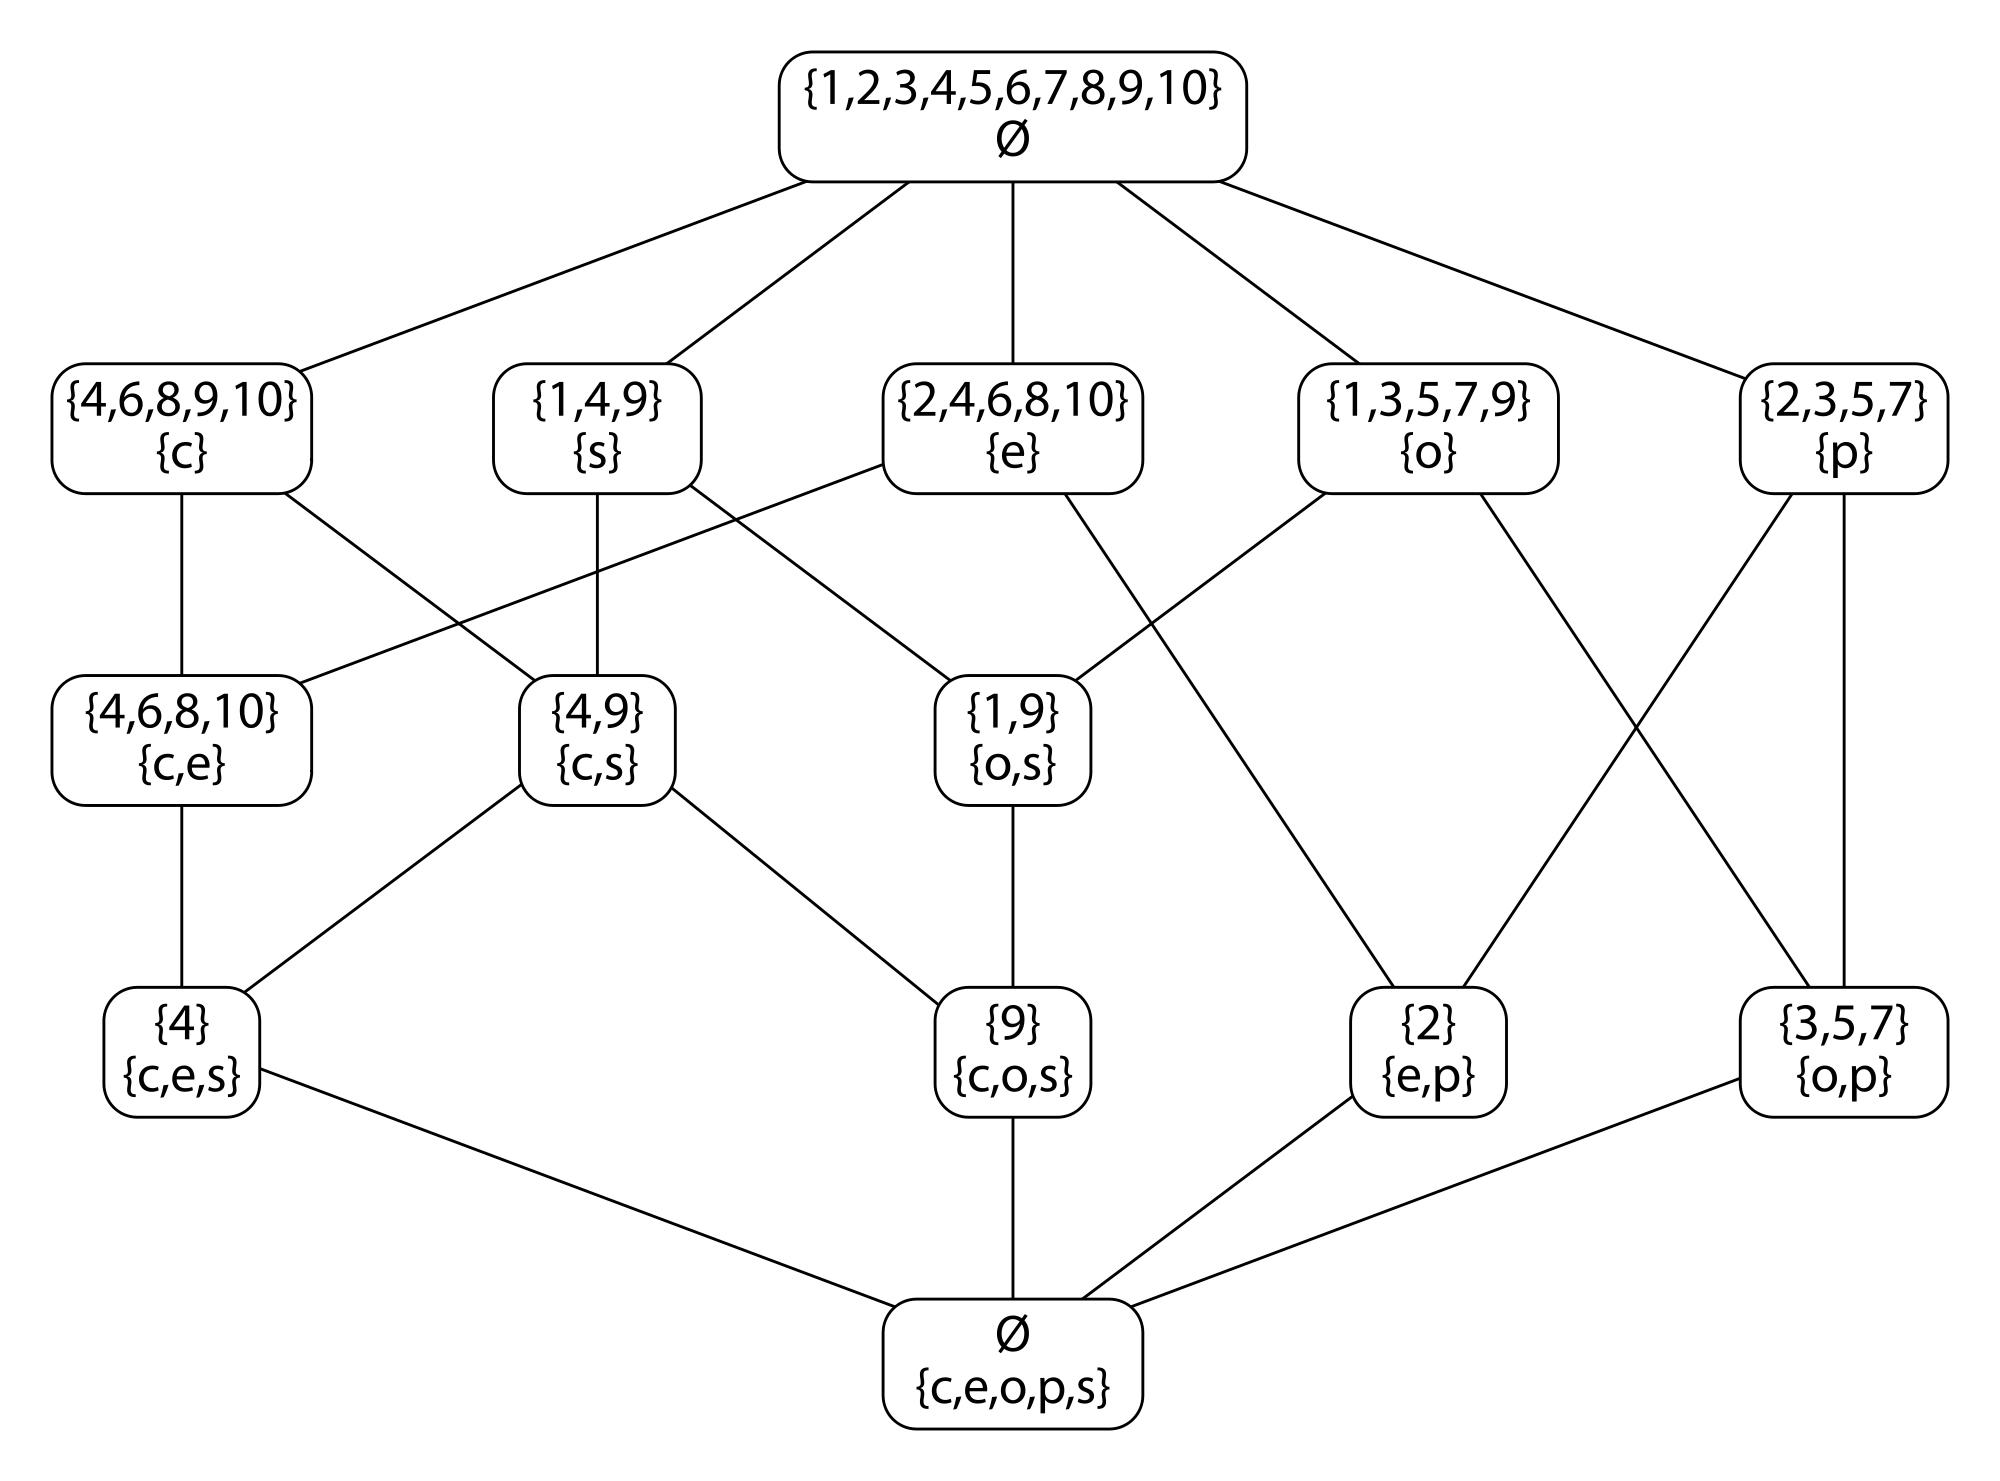
\includegraphics[width=\linewidth]{./images/fcaExample}
\end{figure*}

A Hasse diagram is a special graph where the vertices represent formal concepts and edges represent the relation $\le$ among the formal concepts. An egde between formal concepts $C_i$ and $C_j$ is drawn, when $C_i \le C_j$ and there does not exist a formal concept $C_x$ such as $C_i \le C_x \le C_j$. To increase the readability, the nodes are ordered in layers. The concepts in top are more general, the concepts in the bottom are the more specific. There are two special concepts: supremum and infimum. The supremum is vertex node in the top and the attributes in its intent are those which are present in all objects. The infimum is the vertex in the bottom and the objects in its extent are those which have all attributes. \\

After this general introduction, we will describe in the next section how we can apply FCA to Information Retrieval.

\subsection{Application for Information Retrieval}

The examples depicted in table \ref{table:example} and figure \ref{figure:example} are only exemplary. How did FCA affected the real world? According to Poelmans et al. has been FCA "applied in many disciplines such as software engineering, knowledge discovery and information retrieval" \cite{Poelmans2013} and they did two comprehensive surveys on the application of FCA \cite{Poelmans2013, Poelmans2013b}. \\

Carpineto et al.\cite{Carpineto2005} describe the start of FCA in information retrieval:

\begin{quote}
In the 80's, basic ideas were put forth - essentially that a concept can be seen as a query (the intent) with a set of retrieved documents (the extent) and that neighbor concepts can be seen as minimal query changes."
\end{quote}

This means that the objects are documents and the documents are treated as a set of words. An attribute means that a word occur in this documents. In this simple form, this has a major drawback because it is not possible to we weight terms or for instance to rank among documents with the same attributes. How the user can navigate through the lattice is described in later sections XX-INSRT REF.\\

The different algorithms to create concept lattes or an in-depth analysis of FCA for text mining are not covered in this thesis. The interested reader is guided to study the work from Carpineto and Romano \cite{carpineto2004concept} for an detailed introduction. \\

Selected work of IR+FCA is discussed in the related work section. Before we do this, let us get to know some design principles to discuss the work in regard to those principles.

\section{Interface Design}

The interaction from the user with the system is what exactly matters to the user. The interaction of humans with computers own research area (human-computer interaction) and one of its pioneers is Ben Shneiderman. In the following, two principles from him will be presented: The "Eight Golden Rules of Interface Design" and the "Visual Information Seeking Mantra".

\subsection{Eight Golden Rules of Interface Design}

This rules are genreal advices for user interface designers which should apply to all interfaces. Ben Shneiderman et al. present this rules in their book \cite{Shneiderman2010}. The rules are explained with own remarks. \\

\begin{itemize}
	\item Strive for consistency: Use similar actions in similar situations. Use identical terminology, colors, fonts etc. throughout the system.	
	\item Cater to universal usability: Design for the needs of a diverse user group (skill level, age, gender)
	\item Offer informative feedback: Give system feedback for every action.
	\item Design dialogs to yield closure: Sequences of actions should be grouped. Give feedback on completion of a group.
	\item Prevent errors: Design the system that the user cannot even do errors in the first place. But if she does some, offer instructions how to recover.
	\item Permit easy reversal of actions: Actions should be undone. This gives the user confidence to explore the system.
	\item Support internal locus of control: The user should think that she is in charge of control.
	\item Reduce short-term memory load: Reduce the number of things the user has to keep in mind while using the system.
\end{itemize}

As you can see, the rules are open to interpretation. There exits alternative principles for instance: Donald Norman's Design Principles \cite{Norman2013} or Jakob Nielsen's "10 Usability Heuristics for User Interface Design" \cite{Nielsen1995}. \\

This principles can be applied to all user interfaces. In the next section, design principles will be presented where the user views a large collection of items.

\subsection{Visual Information Seeking Mantra}

The visual information seeking mantra (the Mantra) was introduced by Ben Shneiderman \cite{Shneiderman1996} and are based on his experience with past projects. Albeit the Mantra was intended to be a "descriptive and explanatory" \cite{Card1999}, "in effect, the Mantra has become a prescriptive principle for many information visualization designers", write Craft and Cairns \cite{Craft2005}. \\

The Mantra describes user interface design principles for systems when the "users are viewing collections of items, where items have multiple attributes" \cite{Shneiderman1996}. The starting principles are: overview first, zoom and filter, then details on demand. They will be explained below and added by three other principles. \\

\begin{itemize}
	\item Overview: Gain an overview of the entire collection.
	\item Zoom: Zoom in on items of interest
	\item Filter: Filter out uninteresting items.
	\item Details-on-demand: Select an item or group and get details when needed.
	\item Relate: View relationships among items.
	\item History: Keep a history of actions to support undo, replay, and progressive refinement.
	\item Extract: Allow extraction of sub-collections and of the query parameters.
\end{itemize}

Some task needs more explanation which I will give in the following with help from related literature.

\subsubsection{Zoom and Filter}

This task are responsible for reducing the complexity of the data collection. 'Zoom' means that the user focuses on items she wants to see. 'Filter' means that she can hide items which are not interesting for her.

\subsubsection{History}

It is important to give the user the possibility to easily recover from mistakes. In addition, "it is rare that a single user action produces the desired outcome. Information exploration is inherently a process with many steps, so keeping the history of actions and allowing users to retrace their steps is important." writes Shneiderman \cite{Shneiderman1996}.

\subsubsection{Extract}

Once interesting objects are found, the user should have the possibility to extract them from the system. Shneiderman describes printing, emailing or saving the item to the disk as 'extraction'.

\subsection{Final Remarks}

Only two, very famous design principles were presented here. The are a lot of different alternatives to choose from. There is a lot of interpretation of those guidelines involved. In addition, every system is different and has different requirements. So it is important to threat them with care, but they can help to develop an interface. \\

The presented ideas base mostly on the experience of one person: Ben Shneiderman. The huge number of citations show that his work is influential for a lot of people. But this is not real science. Craft and Cairns \cite{Craft2005} are calling for empirical justification of the Mantra. This is an indication that human-computer interaction is only at the start point - there is a still a lot of research to do.

\chapter{Related Work}

After giving a background in formal concept analysis in general advices we are reviewing the state of art in visualizing concept lattices.

\section{Full Hasse Diagrams}

The traditional, static visualization of concept lattices are Hasse diagrams as describes in XX. Eklund et al. \cite{Eklund2004} conducted user studies and proclaim that non-FCA-experts can read Hasse Diagrams if you fine-tune the Hasse diagram. For instance by choosing appropriate colors, symbols and positioning of the vertices. \\

But in the domain of information (document) retrieval you get formal contexts with a lot of objects. Those Hasse diagrams scale very bad for large concepts lattices. Kuznetsov et al. \cite{Kuznetsov20072}  describe this resulting visualization: "Representing concept lattices constructed from large contexts often results in heavy, complex diagrams that can be impractical to handle and, eventually, to make sense of." Especially the high connectivity of the graph results in enormous edge crossing. The image \ref{figure:firstVisualizaion} shows the first visualization results with their data set. The software XX was used. \\

\begin{figure*}[h]
\caption{First Visualization of the data set with traditional FCA Software}
\label{figure:firstVisualizaion}
	\centering
	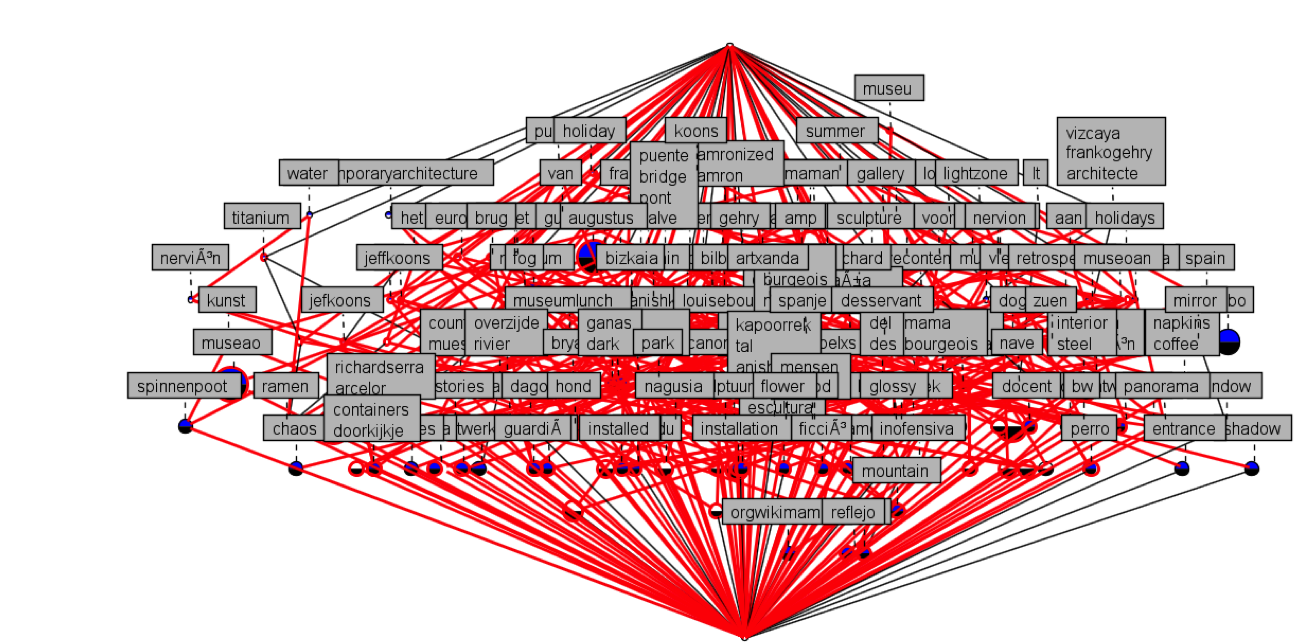
\includegraphics[width=\linewidth]{./images/firstVisualization}
\end{figure*}

The visualization is useless. What can be done to improve the situation? The Hasse can be pruned by reducing the number of vertices. The different techniques are discussed in the next section.

\section{Pruned Hasse Diagrams}

One way to reduce the number of vertices is to compute an "iceberg lattices" \cite{Stumme2002}. They result after the application of the technique originated from data mining "frequent item-set mining" \cite{Agrawal1993}. Only formal concepts are selected which are considers as 'frequent'. A formal concept is frequent if its intent, the set of attributes, is frequent. This approach has some drawbacks. Kuznetsov et al. \cite{Kuznetsov20072} describe them: "One should be careful not to overlook small but interesting groups, for example, “exotic” or “emergent” groups not yet represented by a large number of objects, or, groups that contain objects who are not members of any other group." They propose to only select 'stable' concepts and write "A concept is stable if its intent does not depend much on each particular object of the extent." \cite{Kuznetsov20072}. It is also possible to apply traditional cluster techniques like fuzzy K-Means clustering to FCA \cite{AswaniKumar2010}. \\

	While all these techniques undoubtable reduces the number of formal concepts, it is to question if the results are any helpful. In our case of information retrieval, we apply FCA to explore the data and get insights about it. When pruning the nodes, you are losing many data relationships, many formal concepts and, consequently, the "power" of FCA as exploratory technique is significantly reduced. When we deal with large concepts lattices, the resulting visualization can only contain a very low percentage of formal formal concept. In the year 2015, the question is not how can I analyze 16 formal concepts as in XX - it is more how can I analyze 16000 formal concepts. For this tasks, this approach is not appropriate. \\
	
	Another idea are nested line (/Hasse) diagrams. There the attributes of a formal context are split and a hierarchical order is built up. For instance if you just have two layers: You built up the Hasse diagram for the first layer. And inside the vertex there are is the Hasse Diagram for the second layer and so on. An example is shown in XX. \\
	
But how to split the groups? First - manual selection: This is not doable. Second - automatically selection. This can be done for instance by the stability measurement. But his has the sample like described above. But now you do not remove the concepts but 'hide' them. But overall this approach has not found many friends. Maybe it is because it is very complex and not doable for users. And overall a lot more graphs are added and this can be very distracting. For our case this is not doable because we just have to many formal concepts. There exist even over 1000 Formal Concepts with the highest stability measure of 100\%. \\

The reduction of formal concepts and changing the structure of the lattice maybe useful for different applications, for us there are not. In the next section we will see a technique that is used by a lot of applications in the IR field.

\section{Local View}

Instead of showing the full Hasse diagram, the user can see a local view on the lattice. We will give an overview about the basic idea and applications before we review one real-world application in detail. \\

\subsection{Basic Idea}
The interface is always focused on one formal concept. The user can query the system or navigate through the lattice by going up (removing terms) or going down (adding terms). The figure shows the example from the start with the focus on the concept with the attributes. {o,s}. \\ 


Eklund et al. define their navigation method \textit{conceptual neighborhood} \cite{Eklund2009,Eklund2012}. Only directly related stuff is shown and the visualization is very different from a Hasse diagram. \\

To fully explore the whole lattice the user iteratively navigate through the lattice. In the following, first the history is described and then the way how to navigates is described with an example. \\

The idea originated from the information retrieval field and was first proposed by Godin et al. \cite{Godin1989}. The user queries the system and find the corresponding formal concepts. The documents are shown but also neighboring formal concepts are shown. So after the initial query, the user does not have to formulate new queries and can browse the system iteratively. \\

Two underlying information seeking models stand behind his approach. First, user tend to start with a short query and then refine their needs. Hearst \cite{Hearst2009} write  while referring to \cite{Marchionini2006,Bates1990}:
\begin{quote}
	A commonly-observed search strategy is one in which the information seeker issues a quick, imprecise query in the hopes of getting into approximately the right part of the information space, and then doing a series of local navigation operations to get closer to the information of interest
\end{quote}

Second, it easier for the user to choose from suggestions than to formulate a query. Aula writes \cite{Aula2005}:
\begin{quote}
	Considered in cognitive terms, searching is a more analytical and demanding method for locating information than browsing, as it involves several phases, such as planning and executing queries, evaluating the results, and refining the queries, whereas browsing only requires the user to recognize promising-looking links.
\end{quote}

Godin et al. \cite{Godin1993} evaluated their work in comparison to boolean retrieval and hierarchical retrieval and proclaim that "[their experiments] suggests that retrieval using a Galois lattice structure may be an attractive alternative since it combines a good performance for subject searching along with browsing potential." \\

\subsection{Examples}a

Carpineto and Romano picked up the idea from Godin et al. and developed a FCA search engines ULYSSES \cite{Carpineto1995,Carpineto1996}. The user can fine-tune what neighboring vertices are displayed by bounding the information seeking space. For instance the minimal distance between focused vertices and other vertices. Or parents, children. In Figure \ref{figure:ulysses} is a screenshot of the system. \\

\begin{figure*}[h]
	\centering
	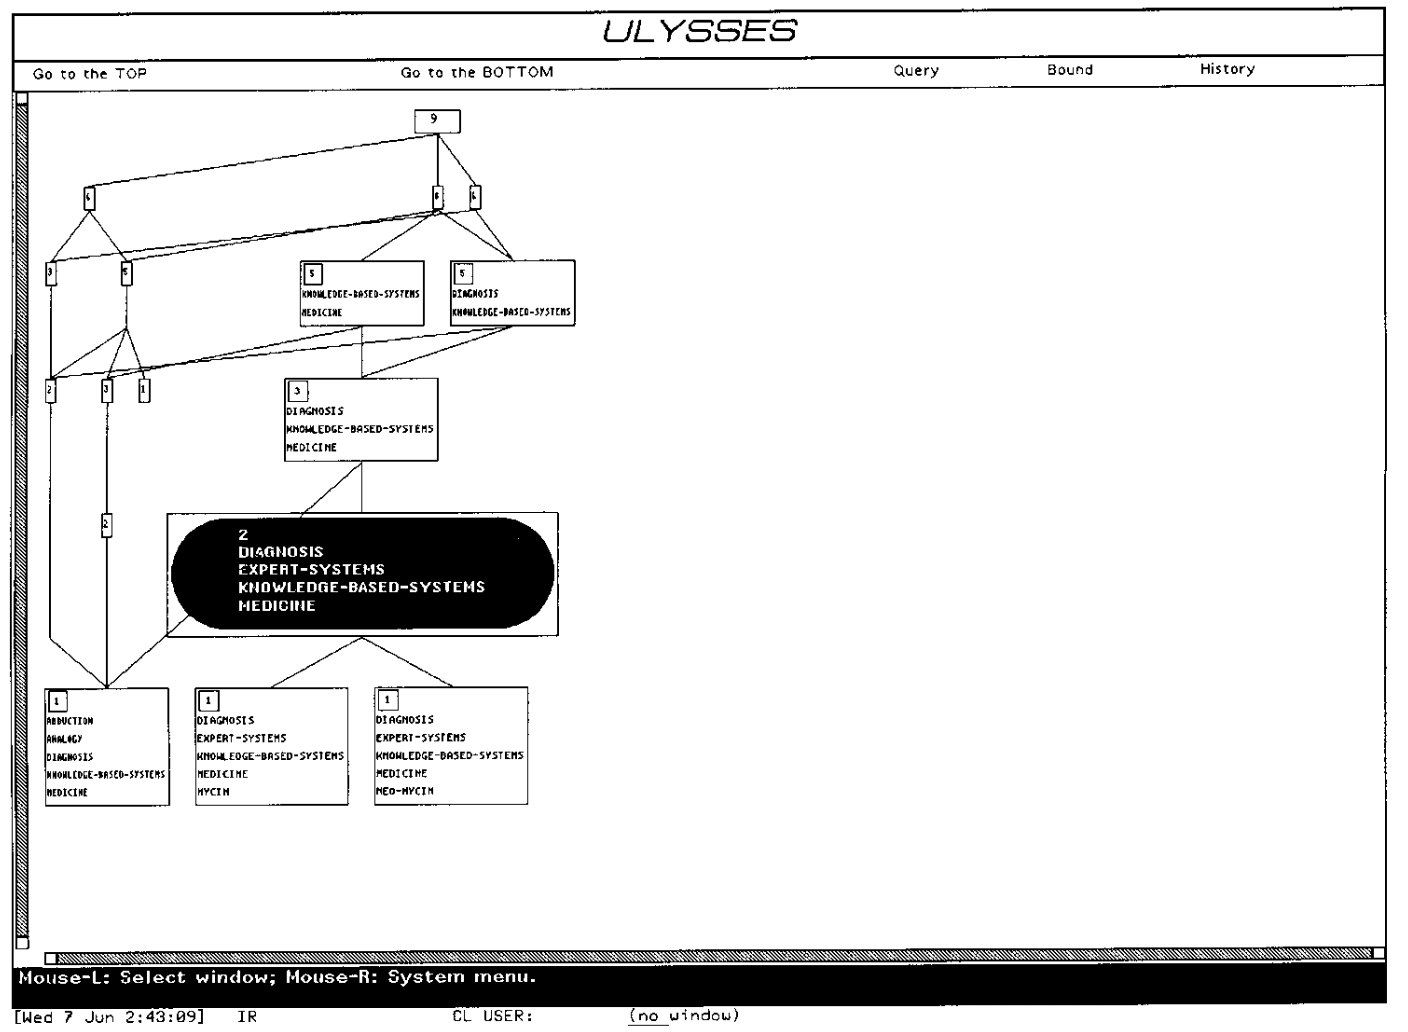
\includegraphics[width=\linewidth]{images/ulysses}
\caption{Display screen of ULYSSES, focusing on the black node \cite{Carpineto1996} }
\label{figure:ulysses}
\end{figure*}

In their following work, CREDO \cite{Carpineto2004}, Carpineto and Romano followed the look of ordinary search engines. The presentation of the concept lattice is not oriented at the Hasse Diagram. It looks more like a folder structure. Shown in \ref{figure:credo}. Nauer and Yannik built CreChainDo \cite{Nauer2009} is built on Credo is a more updated variation. Other works: Koester \cite{Koester2006} and Dau et al.\cite{Dau2008}.\\

\begin{figure*}[h]
	\centering
	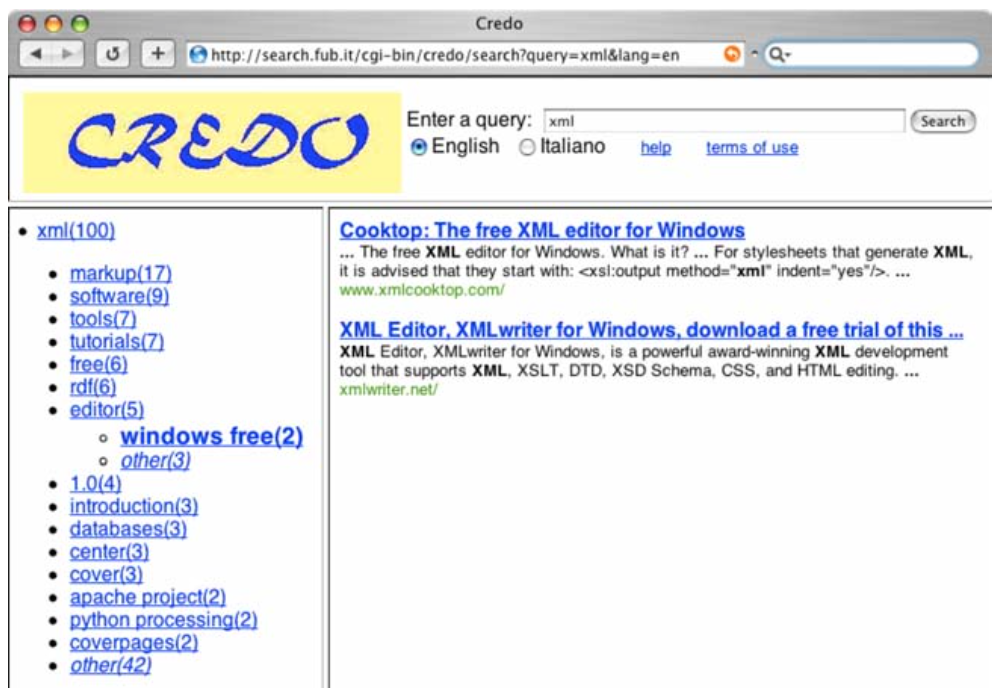
\includegraphics[width=\linewidth]{images/credo}
\caption{Screenshot of CREDO, after query 'xml' and browsing after 'editor(5)' and 'windows free(2)' \cite{Carpineto2004} }
\label{figure:credo}
\end{figure*} 

\begin{figure*}[h]
	\centering
	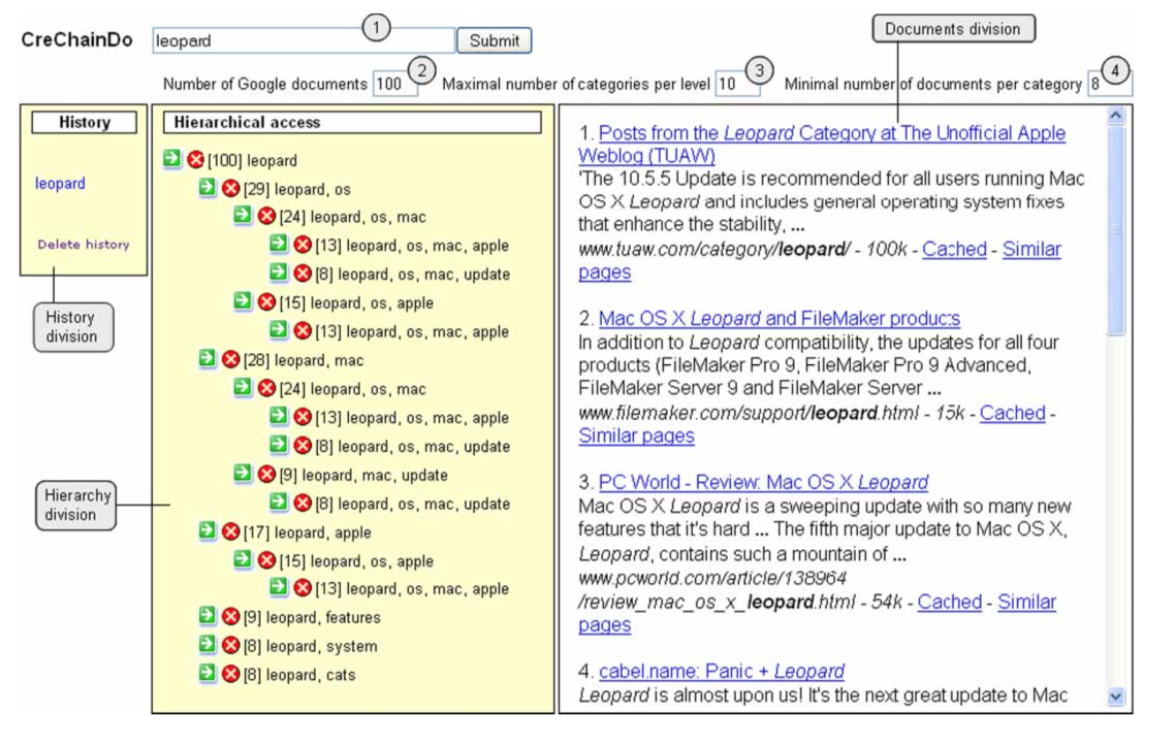
\includegraphics[width=\linewidth]{images/crechaindo}
\caption{Screenshot of CreChainDo, after query 'leopard' \cite{Nauer2009} }
\label{figure:crechaindo}
\end{figure*} 

For now we looked at search engines. Let us review some more genreal approaches.\\


Or the work around Peter Eklund. Eklund et al. applied FCA to email organization\cite{Eklund2004}, image browsing \cite{Ducrou2006,Ducrou2008} and the last work was a 'Virtual Museum of the Pacific' \cite{Eklund2009,Eklund2012} which is accessible on the web \footnote{\url{http://epoc.cs.uow.edu.au/vmp/} - A login is required. You can use. username: filter and password: 45755}. Let us review the museum in-depth because it is very similar to our stuff. \\
 
 \subsection{Review of the Pacific Museum}
 
 If we take the the Mantra (REF XX) we see that some stuff is missing: There is no overview. Or at least there is no overview first. There is details on demand and you zoom into collection an you find interesting. Filter out is really difficult to implement with FCA. It related items are shown. But what there is no way to go back in history. Or to save this document. The problem with the missing is a real problem. It is also in the principle because a history gives the user confident to explore the system. FCA is truly exploratity technique and requieres a lot of confidence to do it. That this is a real problem can be seen in the user studies they conducted. LALA
 
 And for the search interface, it can be approved by sticking to the design of modern search engines.
 
 \begin{figure*}[h]
\label{figure:pacific}
	\centering
	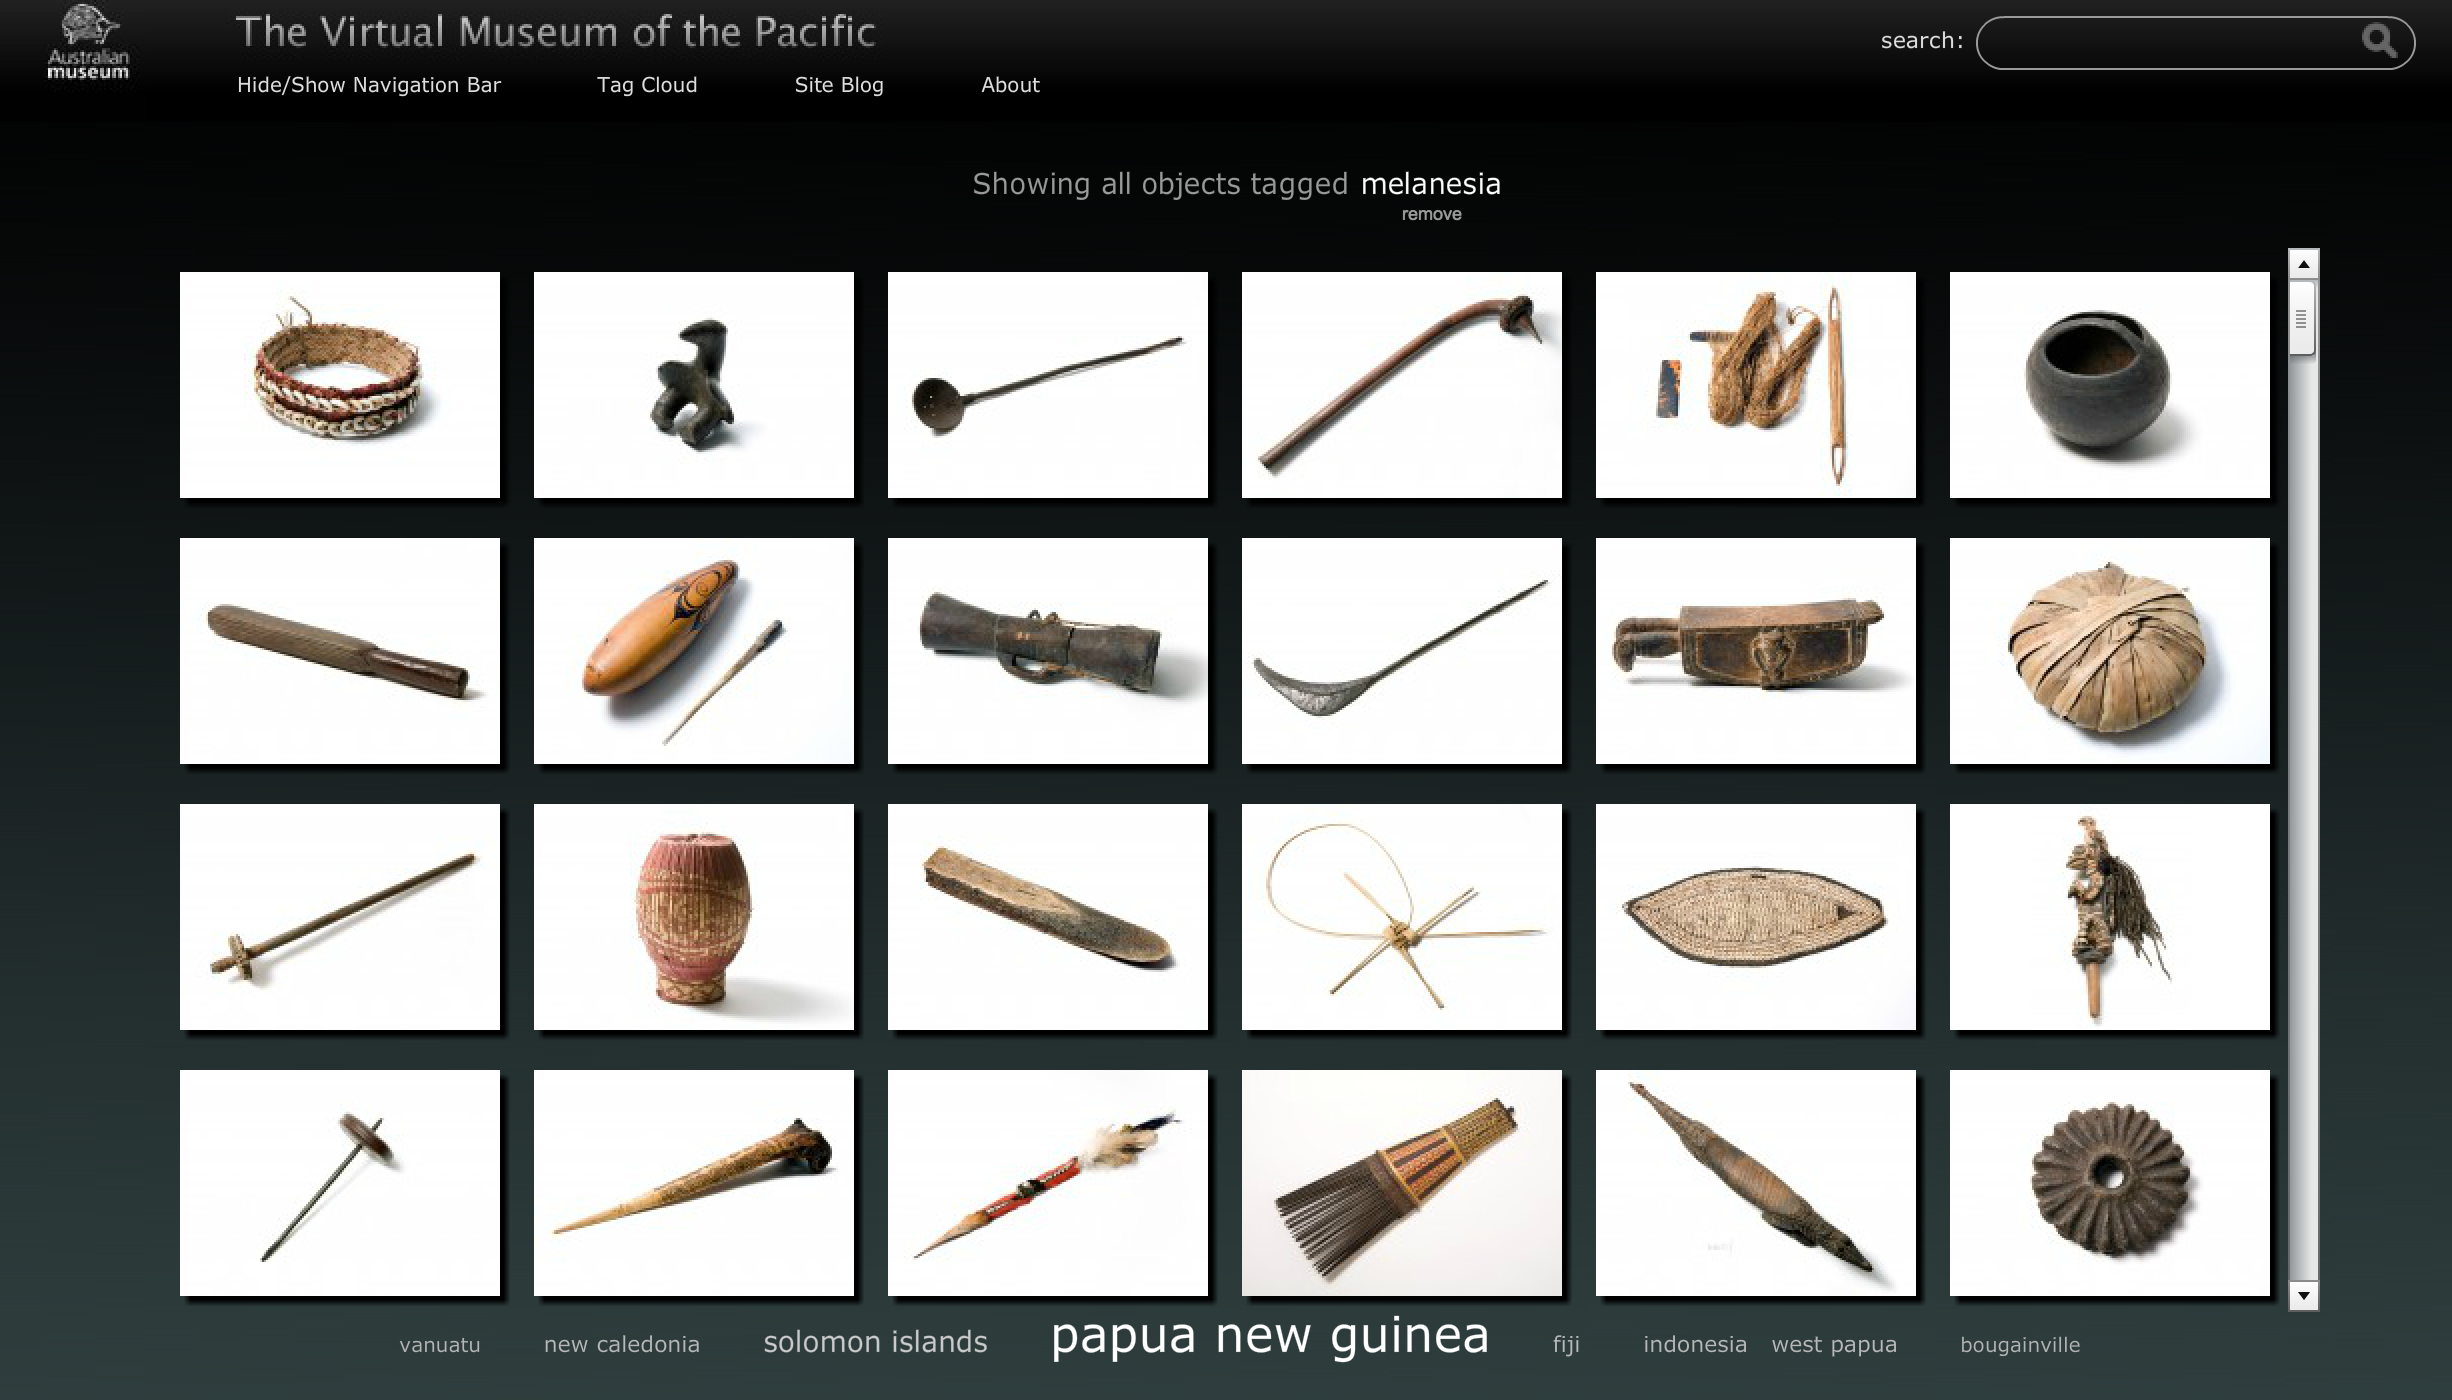
\includegraphics[width=\linewidth]{images/pacific}
\caption{Screenshot of 'Virtual Museum of the Pacific', focus on concept 'melanesia'}
\end{figure*}
 
 

 
 After identifing this problems, we want to built on it. but before that let us review some non-fca-based related work.


\section{Facted Browsers}

DT are similar. But not for text mining. 

\section{Conclusion}

FCa is gre

 he has percpectives: also a taxonomy. But by introducing  manual taxinomy may be useful for the user, but it makes the use of FCA useless because there exist better approaches for this kind of stuff (see below)











\chapter{Fancy FCA 1.0}

\section{My Idea}

We just want to find out if our approach, treating FCA as internal data structure and offering an user search interfaces + guidance (type ahead, showing neighboring concepts), is helpful for human scholars. This can be answered with a usability study.

\subsection{Interface}

The interface should look like a modern search interface. That is why the search bar is on the top. The results are shown in a vertical list. 

The stuff to go deeper is shown as a word cloud but with a scrict seperation between the bubbles. The thought process: Why this interface? An alternative view for instance a list of words. with or without indicating the number of stuff would impose a strict hierachrical order. terms on the top would be clicked a way often. while this approach is not perfect it tries to create a equal way to interact.

Breadcrumbs are under the sreach bar. They are used in most modern website for navigtion.

\section{Implementation}

I will describe important parts of the implementation here.

\chapter{Evaluation of the User Interface}

The design of an interface is highly subjective. User studies can help to evaluate an interface but computer scientists are not experts in human studies and Zobel \cite{Zobel2004} proclaims: "Far too many human studies in computer science are amateurish and invalid." Nevertheless, I tried to be as scientific as possible to conduct human studies even with strict resource limitations. \\

We will present fundamentals of user studies first and then describe our experiments.

\section{Fundamentals}

A small introduction into this field from the computer science perspective gives Hearst in his book on User Search Interfaces in Chapter 2. \cite{Hearst2009}. A comprehensive guide into the "Methods for Evaluating Interactive Information Retrieval Systems with User" gives Kelly \cite{Kelly2007} . The interested reader is advised read those papers because we will only scratch the surface. \\ 


I will describe the idea of the experiment first and refer to literature to illustrate my choices, I will describe the process of the experiment, and after that explain and evaluate the outcome of the results.

\subsection{Introduction}
  If we walk about an evaluation, it is important to make clear what what aspects are evaluated. Hearst writes \cite{Hearst2009}:
  \begin{quote}
  Search interfaces are usually evaluated in terms of three main aspects of usability: effectiveness, efficiency, and satisfaction, which are defined by ISO 9241-11, 1998 \cite{ISO} as:
\begin{itemize}
	\item Effectiveness: Accuracy and completeness with which users achieve specified goals.
	\item Efficiency: Resources expended in relation to the accuracy and completeness with which users achieve goals.
	\item Satisfaction: Freedom from discomfort, and positive attitudes towards the use of the product.
\end{itemize}
These are the criteria that ideally should be measured when evaluating a search user interface."
\end{quote}

It is important to distinguish between the terms 'experiment' and an 'evaluation'. Kelly \cite{Kelly2007} writes: "Evaluations are conducted to assess the goodness of a system, interface or interaction technique and can take many forms [..]. Experiments have historically been the main method for interactive system evaluation, but experiments can also be conducted to understand behavior" and she continues: "Two important characteristics of experiments are that there are at least two things being compared (e.g., system type) and that some manipulation takes place." She further writes:
\begin{quote}
"In some types of [interactive information retrieval] studies only a single system is evaluated. This is a weaker form of evaluation since it is not possible to demonstrate how much better users perform or how different their behaviors and inter actions are since there is no point of comparison. Traditional usability tests are examples of this type of evaluation. Traditional usability tests are usually conducted with a single version of a system, with the goal of identifying potential usability problems."	
\end{quote}

In this thesis, only the usability of the system is evaluated to find usability problems - we do not conduct an experiment. Experiments would be helpful to further investigate the impact of this work but exceed this thesis.

\subsection{Categories of User Studies}
Hearst \cite{Hearst2009} categorizes user studies as follows.

\subsubsection{Informal Usability Testing}
Hearst \cite{Hearst2009} describes the process shortly as "Showing designs to participants and recording their responses". It is often used in short iterative cycles to quickly evaluate a design.

\subsubsection{Formal Studies and Controlled Experiments}
Hearst \cite{Hearst2009} says that it is a "form of controlled experiments aim to advance the field's understanding of how people use interfaces, to determine which design concepts work well under what circumstances, and why."  In contrast to informal studies, it is important to isolate factors and not threat the whole system as a black box. Using eye tracker in a laboratory with 2-way windows is one example.
	
\subsubsection{Longitudinal Studies}
"A longitudinal study tracks participant behavior while using a system over an extended period of time, as opposed to first-time usages which are what are typically assessed in formal and informal studies"

\subsubsection{Log Analysis}
In contrast to the studies above, this focus only on logs of real user interaction. Drawing conclusions from the analysis of Google Search Queries is an example.

\subsubsection{Bucket testing (A/B Testing)}
The traffic to a particular website is split and alternative view. It is evaluated how the users of the alternative website reacts to he new site. For example: Amazon changes its search filters and evaluates if the users buy more.

As you can see, this is only a small categorization and Kelly describes in her work the different approaches more in detail. Because a complete coverage of this topic would exceed this thesis, only some parts are covered here. 

\subsection{Data Collection Techniques}

There exists several techniques to collect data from participants besides from interaction logs. We will describe two more here which are inexpsenvie and do not requier special, expensive euipment or are heavily time-consuming..

\subsubsection{Questionnaires}

A questionnaire comprises a set of questions and is cheap and fast way to gather information from people. Kelly et al. \cite{Kelly2008} describe two types of questions as follows:

\begin{quote}
	Questionnaires can be comprised of closed questions, open questions or a mixture of both. \textit{Closed questions} are questions that provide a fixed set of responses with which subjects must respond. It is common practice for usability questionnaires to include closed questions in the form of statements such as, the system was easy to learn to use. Subjects are typically provided with 5–7-point Likert-type scales for responding, where one scale end-point represents strong agreement and the other represents strong disagreement. [..] \textit{Open questions}, on the other hand, do not provide a response set and subjects are able to provide any type of response they feel is appropriate. 
	\end{quote}

Questionnaires can be done with pen-and-paper, online and in an interview session. Kelly et al. \cite{Kelly2008} conducted research on different ways to elicit responses from the participants. Their results suggest that "the post-system questionnaire takes the form of an interview for closed questions, followed by pen-and-paper or electronic mode for open questions." \cite{Kelly2008} \\ 

Hornbæk and Law did a well respected meta-analysis of usability studies and as one of their conclusions they "recommend that standard questionnaires be used when possible, given their higher reliability, and that the more complex effectiveness measures be used when feasible (as they are more likely to give information that cannot be obtained by measures in the other categories)." \cite{Hornb2007} 

\subsubsection{Thinking Aloud}

Kelly \cite{Kelly2007} writes by referring to Ericsson and Simon \cite{Ericsson1993}: "The think-aloud method asks subjects to articulate their thinking and decision-making as they engage in [interactive information retrieval]". The comments from the participants have to be collected. Either by recording the session or by taking notes. It is hoped that the conductors can learn from the thinking process of the participant. There exist variations like that the participant should not always report because it can be exausting, challening and akwards to report all the time. Called "Spontaneous and Prompted Self-Report" the participant is encourges to report a some points or when he wants to do it.

\subsection{Tasks}

The particpants can specific instructions what to do in the experiment. They can be very concrept or vage formulated. There exists studies which show that there is a correlatin betwwen number of different task and found design errors.

\subsection{Participants}

It is important to reduce a structural bias of an experiment. Zobel \cite{Zobel2004} mentions that "the sample of human subjects should be representative (a class of computer science students may not be typical of users of mobile devices)". We tried to vary the users or at least focus on human scholars because that is the user group that is important for our stuff.


\section{1. Test}

We stick to their advice and use the USE questionnaire \cite{lund2001measuring} which was (partly) used in the investigation from Kelly et all. \cite{Kelly2008}.


\subsection{Hypothesis}

The interface is useful for the human scholars and they like the interface. It offers rich possibilities for the users to navigate along the different documents. Because of the similarity to popular search engines, they know how to use it. But there some stuff that is not implemented yet that they would like to see.

\subsection{Evaluation Design}

Because of our restricted resources, an informal usability study is the most attractive choice for us. The logs of the system are recored and can evaluated in future, but because of the long-term duration, they cannot be evaluated in this thesis.
\section{Results}

\section{Conclusions}

\chapter{Fancy FCA 2.0}

\blindtext

\chapter{Discussions}

\blindtext

\chapter{Conclusions}

\blindtext

\newpage

\bibliographystyle{plain}
\bibliography{biblography}
\end{document}